
{\color{blue}
\section{Non linearity and impact on CMB polarization measurements}
\label{sec:cmb}

Detecting CMB polarization $B$ modes is one of the major goals of modern
cosmology. However, due to the faintness of the expected signal, systematic
effects must be controlled to challenging low levels. In this context, the
knowledge of instrumental characteristics is one of many parameters that must be
well known. Linearity of the detector response is one of these,
and this section addresses its impact on measurements.

KIDs are presented in more details in Sect.~\ref{se:kids}. For now, we model
them as total power detectors placed right after a perfect polarizer whose
transmission direction makes an angle $\alpha$ w.r.t the sky local reference
axis (e.g. the longitude meridian). At each time, they therefore measure a
combination of the Stokes parameters $I$, $Q$ and $U$ of the total incident
radiation. If $\phi$ is the input flux on the KID, to first order, the non
linearity of the KID response can be described by a parameter $\epsilon$ such
that the measure $m=\phi + \epsilon\phi^2$. In the following, we focus on the
extra contribution

\begin{eqnarray}
\Delta m &=& \epsilon\phi^2, \nonumber \\
&=& \epsilon(I+Q\cos2\alpha+U\sin2\alpha)^2, \nonumber\\
 &\simeq & \epsilon I^{2} + 2\epsilon IQ\cos2\alpha + 
2\epsilon IU \sin2\alpha,\nonumber\\
&& + \mathcal{O}e^{i4\alpha}.
\label{eq:eq-NL}
\end{eqnarray}

In the following, we assume that the map making is able to discard the terms in
$4\alpha$ and to project only the spin-2 quantities. Non linearity couples total
intensity to polarization and creates spurious additional contributions to $Q$
and $U$. In addition to CMB, we must account for the foregrounds. We limit
ourselves to dust thermal emission and synchrotron because they are the two
major polarized foregrounds. Any residual of these emissions on the final map
will bias the estimates of the power spectra. While the performances of some
component separation is not the subject of this paper, we must account for these
residuals in eq.~(\ref{eq:eq-NL}) because they can contribute to a significant
fraction of $\Delta m$. We model them by a fraction of their total power such
that $I = I_{cmb} + \eta I_F$ where $F$ stands for ``foregrounds'' and obtain

\begin{equation}
\Delta m = \Delta I + \Delta Q\cos2\alpha + \Delta U\sin2\alpha\,,
\label{eq:eq-NL1}
\end{equation}

with

\begin{eqnarray}
\Delta I &=& \epsilon\left[I_{cmb}^2 + \eta^2 I_F^2 + 2\eta I_{cmb}I_F\right],\\
\Delta Q &=& 2\epsilon\left[I_{cmb}Q_{cmb} + \eta I_FQ_{cmb} + \eta Q_FI_{cmb} +
\eta^2I_FQ_F\right],\\
\Delta U &=& 2\epsilon\left[I_{cmb}U_{cmb} + \eta I_FU_{cmb} + \eta U_FI_{cmb} +
\eta^2I_FU_F\right].
\end{eqnarray}

\planck has provided the most precise measures to date of all the Stokes
parameters involved in eq~(\ref{eq:eq-NL1}) on the entire sky
\cite{2016A&A...594A..10P}. While there has been evidence of spectral index
variations accross the sky (\todo{dust ?  synchrotron? chekc ref}, it is a good
enough approximation for this work to consider that \todo{$I_S,Q_S,U_s(\nu) =
  XXX^\beta$} and \todo{same for dust and add ref}. We consider observations at
70\,GHz where synchrotron is the dominating foreground, observations at 353\,GHz
where dust is taking over, but in each case, we keep the two components. We
build maps of $\Delta I$, $\Delta Q$ and $\Delta U$, mask the Galactic plane for
all latitudes between $\pm 20^\circ$ and compute the power spectra of these maps
using \spice\ \citep{2004MNRAS.350..914C}, an angular power spectrum estimator
that corrects for an incomplete sky coverage. Results are presented on
Fig.~\ref{fig:spice_cl}. Interestingly, as soon as $\eta < XXX$ at 70\,GHz and
$\eta<YYY$ at 353\,GHz, the foreground residuals have negligible impact compared
to the $I_{cmb}Q_{cmb}$ and $I_{cmb}U_{cmb}$ terms in the $\Delta m$ budget. In
order to set an upper limit to the non linearity $\epsilon$ that we can
tolerate, we request $C^{BB}_\ell(\Delta m)$ be smaller than \todo{TBD}. In the
case of a tensor to scalar ration $r$ of $10^{-2}$, $10^{-3}$ \todo{..., this
  leads to XXX}. In the next section, we show that KIDs are expected to meet
these requirements.


\begin{figure}[h]
\center
\includegraphics[scale=0.5]{Figures/cmb_power_spectra.eps}
\caption{Power spectra for spurious temperature and polarization anisotropies of
  eq.~(\ref{eq:spurious-mapI}-\ref{eq:spurious-mapU}). \todo{mentionner a quelle
    frequence on prend les templates, donner un order d'idee de comment les
    epsilon varient en fonction de la frequence donc...}}
\label{fig:cl2}
\end{figure}





}

%%As can be seen, non linearity biases the three Stokes parameters and couples
%%total intensity to polarization. This particular effect is the most problematic
%%as far as polarization is concerned because $I$ is much larger than $Q$ and
%%$U$. This effect is even more stringent if we consider the contribution of dust
%%to this effect that is even brighter than the CMB at frequencies above 100\,GHz
%%on a significant fraction of the sky. In order to be conservative on the limit
%%to set on $\epsilon$, we therefore consider this term as the leading contributor
%%to the final bias. We take the dust polarization map of \planck\ at 353\,GHz and
%%build the maps of the spurious components of eq.~(\ref{eq:eq-NL}):
%%
%%
%%Using \healpix\ \citep{2005ApJ...622..759G}, we compute the angular power
%%spectra of these additionnal components $\Delta C_\ell^{XY}$ where $X$ and $Y$ are
%%either $T$, $E$ or $B$. From eq.~(\ref{eq:eq-NL}) we see that they will add to
%%the polarized angular power spectra of the CMB proportionnaly to $4\epsilon^2$.
%%
%%
%%
%%To investigate the different modes of CMB polarization we used the HEALPix
%%package \citep{2005ApJ...622..759G} to generate modified power spectra from the
%%spurious polarization maps. They are described by Eq.~(\ref{eq:eq-cl}) and are
%%represented in Fig.~\ref{fig:cl2}.
%%
%%\begin{equation}
%%\Delta C_{l} = \epsilon'^{2} C_{l}^{XX'},
%%\label{eq:eq-cl}
%%\end{equation}
%%Where $\lbrace X,X' \rbrace$ = $\lbrace T,E,B \rbrace$ .\\
%%
%%\begin{figure}[h]
%%\center
%%	\includegraphics[scale=0.5]{Figures/cl2_spurious.eps}
%%	\caption{Power spectra for spurious temperature and polarization anisotropies. The black, blue and red curves indicate the $EE$, $TE$ and $BB$ power spectra. The bottom three red curves represents the $BB$ power spectra for a tensor-to-scalar ratio r = (T/S) = 0.1, 0.01, 0.001.}
%%	\label{fig:cl2}
%%\end{figure}
%%
%%Here we will focus on the leading spurious term $C_{l}^{TE}$ : 
%%\begin{equation}
%%\Delta C_{l}^{BB} = \epsilon^{2} C_{l}^{TE}.
%%\label{eq:eq-cl2}
%%\end{equation}
%%
%%The leakage of temperature into polarization is represented by the coefficient \eps\ of Eq.~(\ref{eq:eq-cl2}). To determine this coefficient, we compute :
%%
%%\begin{equation}
%%\epsilon = \sqrt{\dfrac{r/10}{C_{l}^{TE}}},
%%\label{eq:eq-cl3}
%%\end{equation}
%%
%%they are represented in Tab. \ref{tab:eps-lkg}
%%
%%\begin{table}[h!]
%%\center
%%	\begin{tabular}{|c|c|c|c|}
%%  	\hline
%% 	\backslashbox{$\epsilon$}{$r$} & 0.1 & 0.01 & 0.001 \\
%%	\hline
%%	$\epsilon'$ & 7.90 x $10^{-4}$ & 2.50 x $10^{-4}$ & 7.90 x $10^{-5}$\\
%%  	\hline
%%	\end{tabular} 
%%\caption{Non-linear coefficients related to the leakage of temperature into polarization for scalar-to-tensor ratio r = (T/S) = 0.1, 0.01, 0.001.}
%%\label{tab:eps-lkg}
%%\end{table}
%%
%%In the search of $B$ modes polarization, Planck anticipated a $r$ detection threshold of 0.1 . In Tab. \ref{tab:eps-lkg}, we calculated \eps\ for lower tensor-to-scalar ratio ($(T/S) = 0.1, 0.01, 0.001$). To be able to detect $B$ modes polarization at this level without being contaminated by the leakage of temperature into polarization, the non-linearity coefficient related to the detector and the signal reconstruction must be lower than \eps\ of Eq.~(\ref{eq:eq-cl2}). By satisfying this criteria we can satisfy the other \eps\ from Eq.~(\ref{eq:eq-NL}) because $C_{l}^{TE}$ from dust temperature is the leading spurious term. 
%%
%%To conclude, the study of CMB polarization and the measurement of $B$ modes polarization represent one of the major challenges in modern cosmology. The detection of $B$ modes can be affected by a leakage effect of temperature into polarization. Here we studied the non-linearities that the leakage from dust temperature can create. We have seen that the non-linearity coefficients are ranged between $10^{-4}$ and $10^{-5}$.\\
%%
%%To search for $B$ modes at low tensor-to-scalar ratio, the non-linear coefficient of the detector that we use has to be lower than \eps . In the next section, we will study a systematic effect of KIDs by calculating their non-linearity coefficient, and comparing them to \eps .
